\lstinputlisting[language=bash,basicstyle=\small]{python_codes/fieldstone_94/keywords}

\begin{center}
Code at \url{https://github.com/cedrict/fieldstone/tree/master/python_codes/fieldstone_94}
\end{center}

\par\noindent\rule{\textwidth}{0.4pt}

{\sl This stone was developed in collaboration with Lex Verbrugh}. \index{contributors}{L. Verbrugh}

\par\noindent\rule{\textwidth}{0.4pt}

%%%%%%%%%%%%%%%%%%%%%%%%%%%%%%%%%%%%%%%%%%%%%%%%%%%%%%%%%%%%%%%%%%%%%%%%%%%%%%%%%%%%%%%%

This stone is a simple tool to visualise the UUP07 $V_p$ tomography model \cite{hasp15} in paraview. 
The data is available online at \url{https://www.atlas-of-the-underworld.org/downloads/}.
The file is 230Mb so it is not archived here. 
Simply download it and place in the same folder as the python file. 

The output can be either in a Cartesian domain or a hollow sphere of radius $6371\si{\kilo\metre}$.

\begin{center}
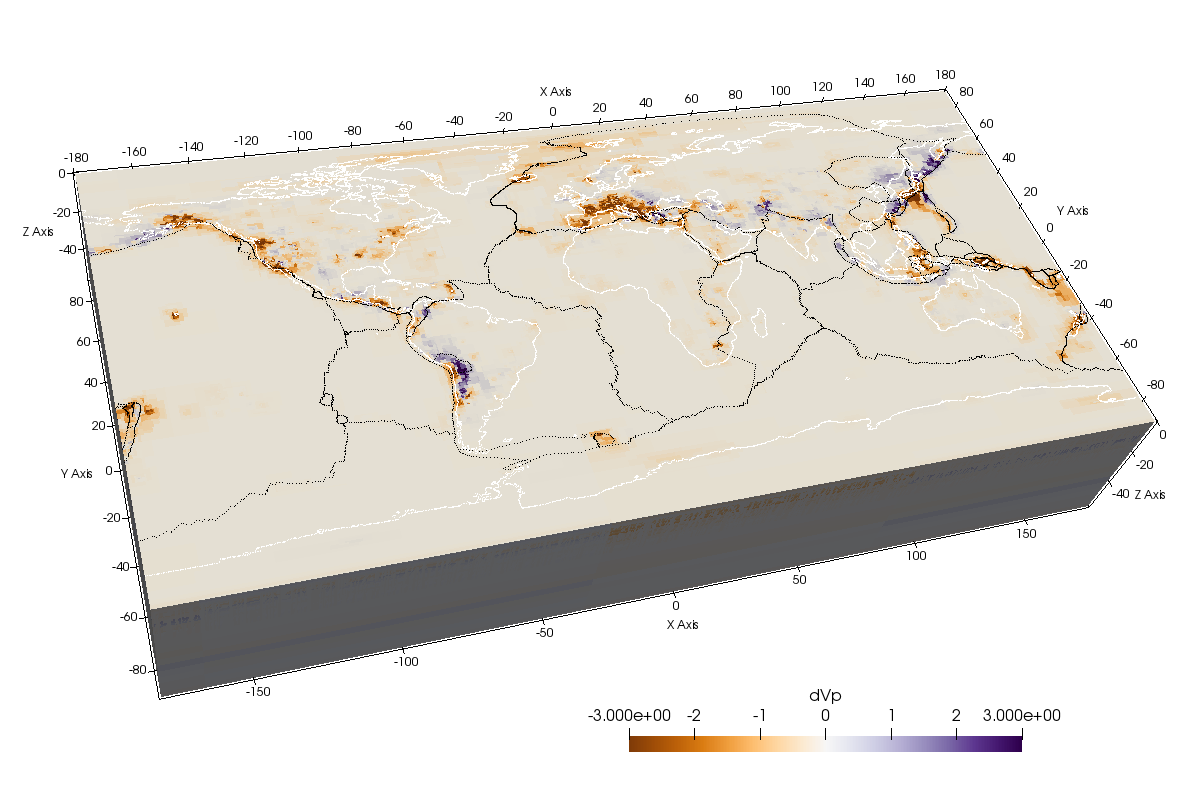
\includegraphics[width=14cm]{python_codes/fieldstone_94/map} 
\end{center}


\begin{center}
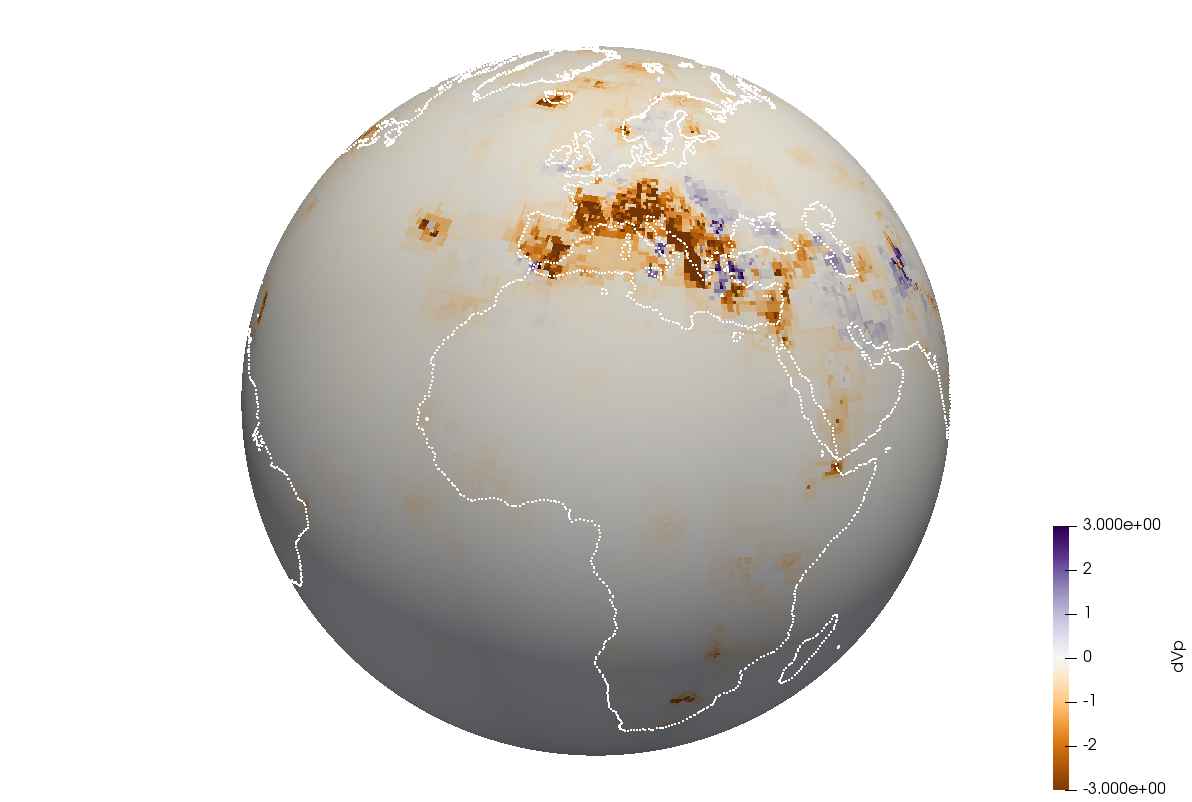
\includegraphics[width=5.7cm]{python_codes/fieldstone_94/sphere1} 
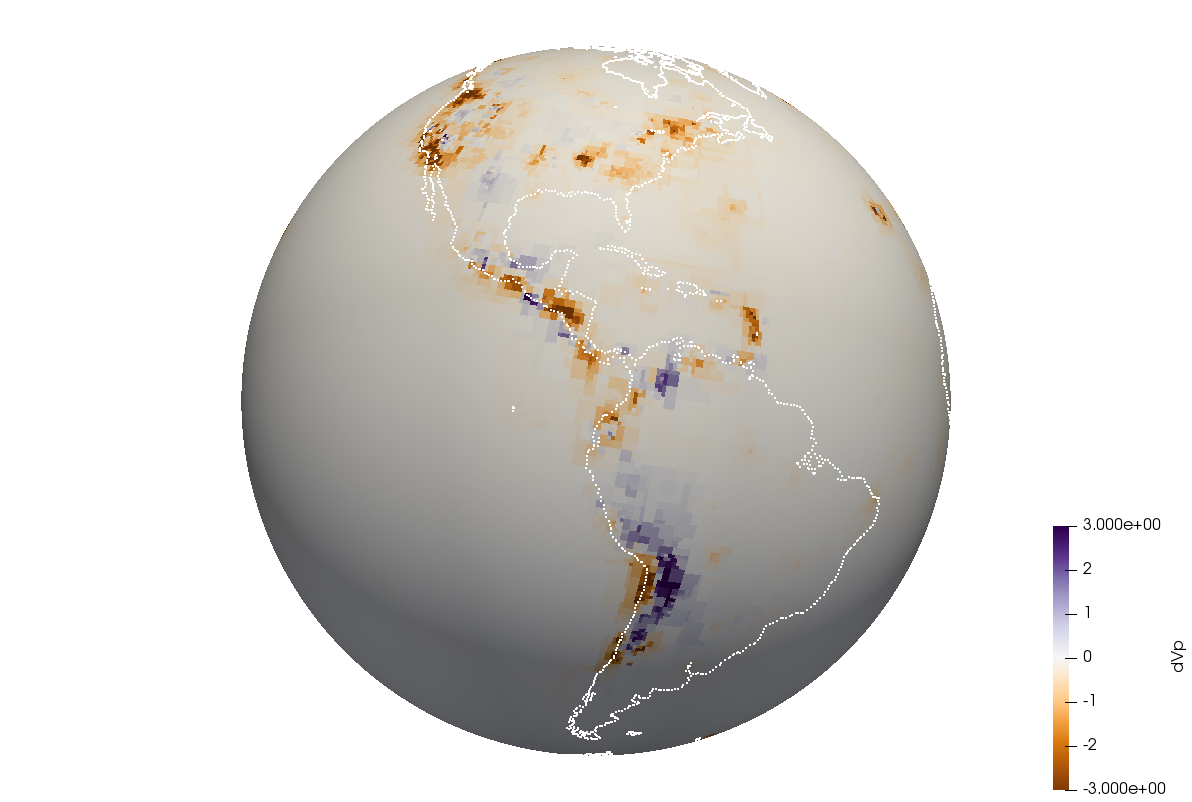
\includegraphics[width=5.7cm]{python_codes/fieldstone_94/sphere2} 
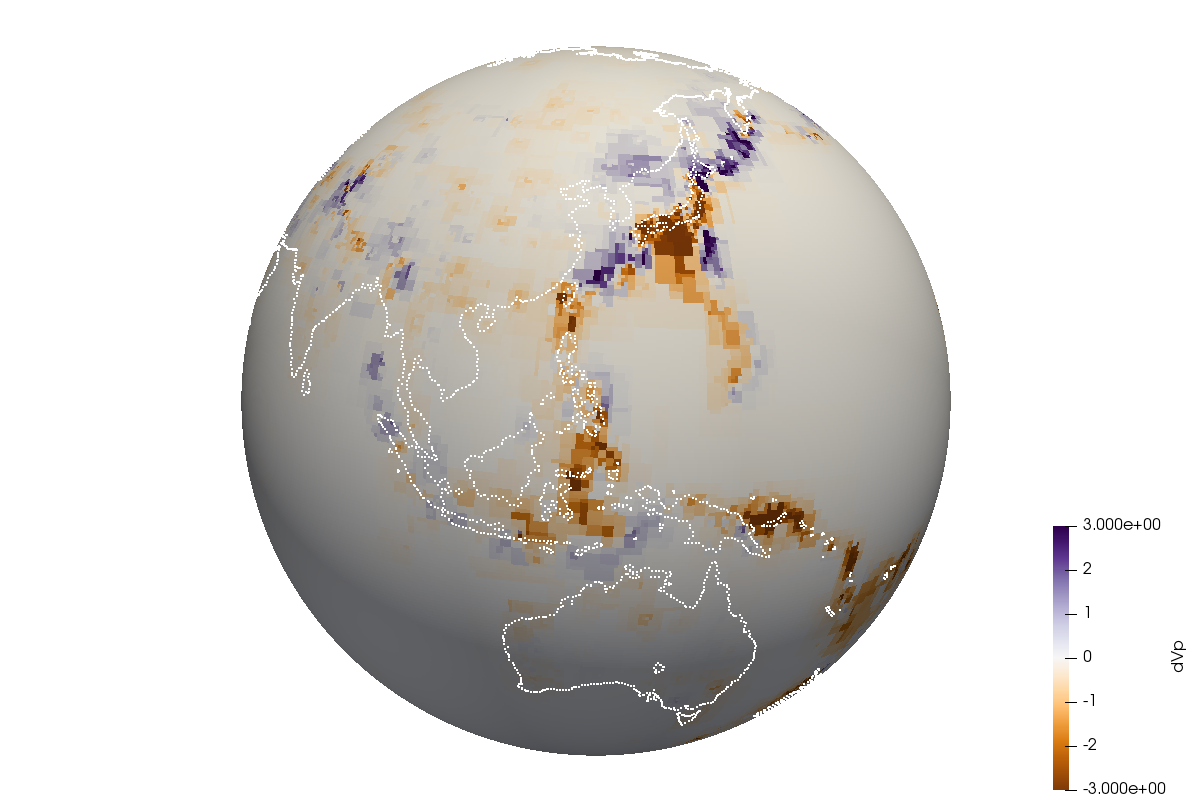
\includegraphics[width=5.7cm]{python_codes/fieldstone_94/sphere3} 
\end{center}


